% ==============================================================================
\section{Módulo de SLAM}
\label{sec:dev_slam}
% ==============================================================================

\subsection{Descripción y alcance}

El módulo de SLAM responde en cada ciclo una pregunta sencilla de plantear y difícil de
resolver, que es dónde está el usuario y hacia dónde mira dentro del mapa que se va
construyendo. Ningún sensor entrega esa respuesta de manera directa. La cámara da la
dirección de los objetos con buena precisión, pero su distancia con mucho error; el
ultrasonido mide distancias exactas, pero solo hacia el frente; y cualquier estimación
de movimiento acumula error con el tiempo. El SLAM junta estas fuentes, lleva la cuenta
de qué tanto se puede confiar en la pose y la entrega a los módulos de Ray Casting y
mapeo. Con ello cubre RF-14 y RF-15.

En TT1 se planteó un SLAM ``simplificado'' basado en un filtro de Kalman extendido
(EKF) \cite{kalman1960, thrun2005probabilistic}, y esa idea se mantuvo, aunque hubo que
precisar la variante. En el EKF-SLAM clásico \cite{smith1990uncertain} el vector de
estado incluye la pose y la posición de cada \emph{landmark}, de modo que la matriz de
covarianza crece con el cuadrado del número de elementos del mapa
\cite{bailey2006slam2}. Los sistemas de SLAM visual como ORB-SLAM
\cite{murartal2015orbslam}, por su parte, siguen miles de puntos característicos y
piden más cómputo del que una Raspberry Pi puede dar mientras también ejecuta la
detección de objetos.

Por eso el estado del filtro contiene solo la pose, $\boldsymbol{\mu} = [x,\; y,\;
\theta]^T$, con una covarianza $\mathbf{P}$ de $3 \times 3$, y el costo de cada ciclo es
el mismo sin importar cuántos objetos haya en el mapa. Los \emph{landmarks} se guardan
en una lista ligera fuera del filtro, cada uno con su posición, su etiqueta (silla,
puerta, mesa, etc.) y el número de veces que se ha visto. Al corregir, el filtro usa el
\emph{landmark} asociado como referencia y suma su incertidumbre de posición, que baja
con cada nueva observación, a la covarianza de la innovación; así no trata a un objeto
recién visto como si su posición fuera exacta. En términos académicos, la variante
corresponde a un EKF de localización con mapeo incremental de apoyo. Se privilegia una
pose barata y estable, y el mapa de ocupación lo refinan después los módulos de Ray
Casting y mapeo con la pose que el SLAM les entrega.

\subsection{Entradas y salidas}

La Tabla~\ref{tab:slam_interfaces} describe las estructuras de datos que intercambia el
módulo, definidas en \texttt{interfaces.py}.

\begin{table}[H]
\centering
\caption{Interfaces del módulo de SLAM}
\label{tab:slam_interfaces}
\renewcommand{\arraystretch}{1.25}
\begin{tabular}{|p{3.3cm}|p{1.6cm}|p{9.6cm}|}
\hline
\textbf{Estructura} & \textbf{Tipo} & \textbf{Contenido} \\
\hline
\texttt{MotionEstimate} & Entrada & Desplazamiento $\Delta d$ (m), giro $\Delta\theta$
(rad) e intervalo $\Delta t$ (s) desde el ciclo anterior. \\
\hline
\texttt{Observation} & Entrada & Rango $r$ (m), dirección $\phi$ relativa al frente
del usuario (rad, positiva hacia la izquierda), etiqueta, desviaciones estándar propias
$\sigma_r$ y $\sigma_\phi$, y banderas que indican si la observación puede crear
\emph{landmarks}, si puede corregir la pose y si es un peligro de piso. \\
\hline
\texttt{SlamOutput} & Salida & Pose $(x, y, \theta)$, covarianza de $3 \times 3$,
marca de tiempo y confianza entre 0 y 1. \\
\hline
Lista de \emph{landmarks} & Salida & Posición, etiqueta, número de avistamientos y
estado (candidato o confirmado) de cada elemento del mapa ligero. \\
\hline
\end{tabular}
\end{table}

Como ejemplo, la salida de un ciclo, tal como la recibe el resto del sistema, se ve así.

\begin{verbatim}
pose: {x: 1.83, y: 0.42, theta: 0.31}
covarianza: [[0.0021, 0.0001, 0.0000],
             [0.0001, 0.0019, 0.0000],
             [0.0000, 0.0000, 0.0007]]
timestamp: 1737657000.231
confianza: 0.94
\end{verbatim}

\subsection{Fuentes de movimiento}

Para la predicción hace falta saber cuánto avanzó y cuánto giró el usuario desde el
ciclo anterior. El módulo \texttt{odometry.py} obtiene ese dato de tres maneras, en
orden de preferencia.

La fuente principal es la IMU BNO055 de Bosch \cite{bno055_datasheet}, conectada al
mismo bus I2C que los ultrasónicos y configurada en su modo de fusión NDOF, en el que
el propio chip combina acelerómetro, giroscopio y magnetómetro. El giro de cada ciclo es
la diferencia entre dos lecturas del rumbo fusionado. Para el avance no se integra la
aceleración dos veces, porque el error crecería con el cuadrado del tiempo; se usa en
cambio la navegación peatonal por estima (\emph{pedestrian dead reckoning})
\cite{harle2013pdr}. Cada paso se detecta como un pico en la magnitud de la aceleración
lineal por encima de 1.8~m/s$^2$, con rearme cuando baja de 0.8~m/s$^2$ y un mínimo de
0.3~s entre pasos, y cada paso suma una longitud configurable, de 0.68~m por defecto. La
IMU también mide la inclinación real de la cabeza, que se usa para la distancia por
plano de piso. Como la orientación del chip dentro del armazón puede variar, se
configura con las posiciones de montaje P0 a P7 de su hoja de datos, y el programa
\texttt{odometry.py --calibrar} identifica, con los lentes puestos, qué eje corresponde
al cabeceo, su signo y su cero.

Si la IMU no responde, el sistema pasa solo al flujo óptico de la cámara. Se eligen
puntos característicos con el detector de Shi--Tomasi \cite{shi1994good}, se siguen
entre cuadros con el método de Lucas--Kanade \cite{lucas1981iterative} y el giro se
calcula con la mediana del desplazamiento horizontal, $\Delta\theta =
\arctan(\overline{\Delta u} / f)$, donde $f$ es la distancia focal en píxeles. En este
modo no se estima el avance.

La tercera fuente solo se usa al procesar videos grabados, que no traen información
inercial. Al flujo óptico se le resta la parte que corresponde al giro, y si lo que
queda supera 1.4 píxeles se considera que el usuario está caminando, con una velocidad
supuesta de 1.1~m/s. Con esto se pueden construir mapas a partir de videos, aunque su
escala depende de esa velocidad.

\subsection{Construcción de observaciones}

La función \texttt{fuseObservations} convierte las detecciones de la cámara y las
lecturas ultrasónicas en observaciones de rango y dirección. La dirección de un objeto
sale de la columna central de su caja y del campo de visión de la cámara. La distancia
se estima con el modelo de cámara estenopeica \cite{hartley2004multiple}:

\[
d_{h} = \frac{f \, H_{\text{típica}}}{h_{\text{bbox}}},
\qquad
f = \frac{W/2}{\tan(\text{FOV}_h/2)}
\]

donde $H_{\text{típica}}$ es la altura típica de la clase (1.65~m para una persona,
0.90~m para una silla o 2.00~m para una puerta, por ejemplo) y $h_{\text{bbox}}$ es la
altura de la caja en píxeles. Si el borde inferior de la caja se ve en la imagen, se
calcula además la distancia al punto donde el objeto toca el piso:

\[
d_{g} = \frac{h_{c}}{\tan\!\left(\alpha + \arctan\dfrac{v_b - H/2}{f}\right)}
\]

con $h_c = 1.55$~m como altura de la cámara, $\alpha$ como su inclinación hacia el piso
(10° por defecto, o la que mide la IMU) y $v_b$ como la fila del borde inferior. El
resultado final es $d_g$, pero acotado entre $0.4\,d_h$ y $1.6\,d_h$, lo que combina la
estabilidad del primer modelo con la mejor precisión del segundo.

Cada observación lleva su propia incertidumbre y el filtro la usa para dar más o menos
peso a cada fuente, sin necesidad de casos especiales. La Tabla~\ref{tab:slam_fusion}
resume las reglas.

\begin{table}[H]
\centering
\caption{Reglas de construcción de observaciones y su incertidumbre}
\label{tab:slam_fusion}
\renewcommand{\arraystretch}{1.25}
\begin{tabular}{|p{4.3cm}|p{2.4cm}|p{1.6cm}|p{5.9cm}|}
\hline
\textbf{Caso} & $\sigma_r$ & $\sigma_\phi$ & \textbf{Uso} \\
\hline
Detección visual con eco ultrasónico compatible & 0.05~m & $3^\circ$ & Rango del
ultrasonido y dirección de la cámara. Corrige la pose y crea \emph{landmarks} con 2
avistamientos. \\
\hline
Detección visual sin respaldo & $0.30\,r$ & $3^\circ$ & Corrige la pose; hacen falta 4
avistamientos para confirmar un \emph{landmark}. \\
\hline
Peligro de piso (hoyo, agua, escalera) & $0.20\,r$ & $3^\circ$ & Va a la capa de
peligros del mapa. \\
\hline
Eco ultrasónico sin detección visual & 0.05~m & $10^\circ$ & Solo actualiza el mapa;
no corrige la pose ni crea \emph{landmarks}. \\
\hline
Objeto en movimiento & --- & --- & Se descarta, porque una persona caminando no es una
referencia fija. \\
\hline
\end{tabular}
\end{table}

Una detección y un eco se toman como el mismo objeto si sus direcciones difieren menos
de $20^\circ$ y sus rangos son compatibles, es decir, si
$|r_{us} - r_{mono}| \leq \max(0.6,\; 0.5\, r_{mono})$.

\textbf{Ecos de pared.} En una primera versión, los ecos que no tenían una detección
visual asociada también creaban \emph{landmarks} y corregían la pose. El problema es que
el punto donde rebota un eco sobre una pared se desliza conforme el usuario camina, así
que no es un punto fijo del mundo, y usarlo como referencia echaba a perder la pose. Al
sacar esos ecos de la corrección, el ATE promedio del banco bajó de 0.53 a 0.27~m. Los
ecos se siguen enviando siempre al mapa de ocupación, porque el extremo de cada rayo sí
cae sobre la superficie que lo produjo.

\textbf{Ultrasonido frontal y validación cruzada.} Los dos MB1232 del prototipo van al
frente, uno sobre cada cristal, separados unos 10~cm y apuntando en la misma dirección
que la cámara (Sección~\ref{sec:dev_prototipo}). Según su hoja de datos son sensores de
haz angosto, con un cono útil de unos $\pm 14^\circ$, y su alcance depende del tamaño
del objeto; alimentados a 3.3~V, como en la Raspberry Pi, detectan a una persona hasta a
1.8~m y una pared hasta a unos 6~m \cite{mb1232_datasheet}. Sobre este montaje se
construyeron cuatro mecanismos.

El primero es geométrico. Cada lectura se convierte a coordenadas polares centradas en
la cámara, tomando en cuenta el desplazamiento lateral de su sensor, antes de
fusionarla. El segundo aprovecha que los dos sensores ven casi lo mismo, pues cuando
ambos detectan el mismo objeto, la diferencia entre sus rangos indica de qué lado está,
con $y = (r_{der}^2 - r_{izq}^2)/2s$, donde $s$ es la separación, y una zona muerta de
5~cm para no reaccionar al ruido.

El tercero es la validación cruzada, que corresponde al Algoritmo 2 de TT1. Si una
detección visual cae dentro del cono y hay un eco compatible, se marca como confirmada
por ambos sensores y toma el rango del ultrasonido, que es mucho más preciso. Si el haz
debería alcanzar al objeto, por su tamaño, su altura y su distancia, pero el eco está
mucho más lejos, la detección se marca como contradicha. Con las puertas el criterio
sirve también para saber su estado, ya que un eco que pasa por el vano indica que está
abierta y uno a la distancia de la puerta, que está cerrada; esto corrige las puertas de
vidrio que la segmentación daba por abiertas. El cuarto mecanismo descarta los ecos del
piso. Cuando el usuario inclina la cabeza, el haz rebota en el suelo; con el cabeceo de
la IMU se calcula a qué distancia lo toca, y esas lecturas se tratan como espacio libre
y no como pared.

Como los dos sensores apuntan al mismo lado, si disparan a la vez cada uno escucha el eco
del otro. Por eso el driver los dispara de forma alternada en un hilo propio, con
100~ms entre la orden de medir y la lectura, como indica la hoja de datos.

\subsection{Predicción}

La pose se propaga con un modelo de arco, en el que el avance se aplica en la
orientación promedio del tramo. Es más exacto que aplicarlo en la orientación inicial
cuando el usuario gira mientras camina.

\[
\theta_m = \theta + \frac{\Delta\theta}{2},
\qquad
\begin{bmatrix} x' \\ y' \\ \theta' \end{bmatrix}
=
\begin{bmatrix}
x + \Delta d \cos\theta_m \\
y + \Delta d \sin\theta_m \\
\operatorname{wrap}(\theta + \Delta\theta)
\end{bmatrix}
\]

El jacobiano respecto al estado y la propagación de la covarianza quedan como sigue.

\[
\mathbf{G} =
\begin{bmatrix}
1 & 0 & -\Delta d \sin\theta_m \\
0 & 1 & \Delta d \cos\theta_m \\
0 & 0 & 1
\end{bmatrix},
\qquad
\mathbf{P}' = \mathbf{G}\,\mathbf{P}\,\mathbf{G}^T + \mathbf{Q}
\]

El ruido de proceso crece con el movimiento, con
$\mathbf{Q} = \operatorname{diag}(\sigma_t^2,\, \sigma_t^2,\, \sigma_\theta^2)$,
$\sigma_t = 0.02 + 0.05\,|\Delta d|$~m y
$\sigma_\theta = 0.035\,\max(|\Delta\theta|,\, 0.01) + 0.3^\circ$. La covarianza
inicial es $\operatorname{diag}(0.01,\; 0.01,\; (1^\circ)^2)$, porque el sistema arranca
en el origen de su propio marco de referencia.

\subsection{Modelo de observación y asociación de datos}

Para un \emph{landmark} conocido en $(l_x, l_y)$, la observación esperada y su
jacobiano son los siguientes.

\[
\delta_x = l_x - x,\quad \delta_y = l_y - y,\quad q = \delta_x^2 + \delta_y^2
\]
\[
\hat{\mathbf{z}} =
\begin{bmatrix} \sqrt{q} \\ \operatorname{atan2}(\delta_y, \delta_x) - \theta
\end{bmatrix},
\qquad
\mathbf{H} =
\begin{bmatrix}
-\delta_x/\sqrt{q} & -\delta_y/\sqrt{q} & 0 \\
\delta_y/q & -\delta_x/q & -1
\end{bmatrix}
\]

Cada observación $\mathbf{z} = [r, \phi]^T$ se asocia con el \emph{landmark} confirmado
más cercano en distancia de Mahalanobis, siempre que esa distancia quede por debajo de un
umbral de compuerta \cite{barshalom2001estimation, neira2001jcbb}.

\[
\boldsymbol{\nu} = \mathbf{z} - \hat{\mathbf{z}},
\qquad
\mathbf{S} = \mathbf{H}\mathbf{P}\mathbf{H}^T + \mathbf{R} + \mathbf{R}_{lm},
\qquad
d^2 = \boldsymbol{\nu}^T \mathbf{S}^{-1} \boldsymbol{\nu} < \gamma^2,\quad \gamma = 3
\]

Aquí $\mathbf{R} = \operatorname{diag}(\sigma_r^2, \sigma_\phi^2)$ viene de la propia
observación y $\mathbf{R}_{lm}$ representa la incertidumbre del \emph{landmark}, con
$\sigma_{lm} = 0.4/\sqrt{n}$~m para un elemento visto $n$ veces. Además, solo se comparan
etiquetas compatibles, así que una silla nunca se asocia con una mesa. Las etiquetas
genéricas, como la de un eco sin clase, son compatibles con todas y toman la etiqueta
correcta en cuanto la cámara identifica al objeto.

\subsection{Corrección}

Si hay asociación, se calcula la ganancia de Kalman y se actualizan la pose y la
covarianza. Para la covarianza se usa la forma de Joseph, que es más estable
numéricamente que la forma simplificada y mantiene a $\mathbf{P}$ simétrica y
semidefinida positiva \cite{grewal2015kalman}.

\[
\mathbf{K} = \mathbf{P}\mathbf{H}^T\mathbf{S}^{-1},
\qquad
\boldsymbol{\mu} \leftarrow \boldsymbol{\mu} + \mathbf{K}\boldsymbol{\nu}
\]
\[
\mathbf{P} \leftarrow (\mathbf{I} - \mathbf{K}\mathbf{H})\,\mathbf{P}\,
(\mathbf{I} - \mathbf{K}\mathbf{H})^T + \mathbf{K}\mathbf{R}_{ef}\mathbf{K}^T
\]

donde $\mathbf{R}_{ef} = \mathbf{R} + \mathbf{R}_{lm}$. Después de cada corrección se
impone un mínimo a la varianza de cada componente ($10^{-4}$~m$^2$ en posición y
$(0.5^\circ)^2$ en orientación). Sin ese mínimo, tras miles de correcciones el filtro
terminaría creyendo que su pose es perfecta y dejaría de reaccionar a observaciones
nuevas, lo cual sería grave si el usuario tropieza o alguien lo mueve.

Si en un ciclo ninguna observación se asocia, no hay corrección y el sistema sigue solo
con la predicción. La confianza que se reporta combina la incertidumbre con el número
$k$ de ciclos seguidos sin corrección,

\[
c = \frac{1}{1 + \operatorname{tr}(\mathbf{P})}\cdot 0.9^{k},
\]

de modo que el módulo de navegación sabe cuándo la pose es menos fiable y puede actuar
con más cuidado, como pide RNF-09.

\subsection{Gestión de \emph{landmarks}}

Una observación que no se asocia con ningún \emph{landmark} confirmado no se tira; pasa
a alimentar el mapa ligero. Primero se proyecta al marco global y se busca un candidato
que corresponda al mismo objeto. La comparación usa la elipse de incertidumbre de la
observación, que es estrecha en dirección y alargada en profundidad, y gracias a ella la
misma silla vista a 2.1~m y después a 2.9~m (con el $\pm 30$\,\% de error de la
estimación monocular) se reconoce como un solo objeto. Si no hay candidato, se crea uno
nuevo.

El candidato se confirma tras 2 avistamientos si tiene respaldo del ultrasonido, o tras
4 si solo lo vio la cámara. Así, un falso positivo de YOLO que aparece en uno o dos
cuadros no se convierte en un obstáculo inventado. La observación que confirma a un
candidato no corrige la pose en ese mismo ciclo, para no contar dos veces la misma
evidencia. Cada vez que el objeto se vuelve a ver, su posición se acerca a la nueva
medición con un factor $\alpha = \max(0.05,\; 1/n)$, que al principio equivale a un
promedio acumulado y, cuando el objeto ya se vio muchas veces, a un promedio móvil. Los
candidatos que no se vuelven a ver en 40 ciclos se eliminan, y dos \emph{landmarks}
confirmados con la misma etiqueta a menos de 0.7~m se funden en uno, ponderando por sus
avistamientos, para deshacer duplicados causados por la deriva.

Por último, la función \texttt{observationsForMap} cambia el rango crudo de cada
observación asociada por la posición consolidada de su \emph{landmark}, con
$\sigma_r = 0.05$~m. Con eso cada objeto deja en el mapa de ocupación una marca firme en
la misma celda, en lugar de una mancha dispersa por el ruido monocular; solo se anclan
los \emph{landmarks} con una etiqueta real. Los \emph{landmarks} confirmados se pueden
guardar y volver a cargar en otra sesión (\texttt{exportLandmarks} e
\texttt{importLandmarks}), y así el filtro puede corregir contra un lugar conocido desde
el primer ciclo.

\subsection{Pseudocódigo del ciclo implementado}

El Algoritmo~\ref{alg:dev_slam} resume un ciclo completo del módulo, tal como quedó en
el método \texttt{EKFSlam.step}.

\begin{center}
\captionof{algorithm}{Ciclo del módulo SLAM implementado}
\label{alg:dev_slam}
\end{center}
\vspace{-1.8cm}
\rule{\textwidth}{0.4pt}
\vspace{-0.9cm}
\begin{algorithmic}[1]

\Statex \textbf{ENTRADA:}
\Statex movimiento \Comment{($\Delta d$, $\Delta\theta$, $\Delta t$)}
\Statex observaciones \Comment{lista de (r, $\phi$, etiqueta, $\sigma_r$, $\sigma_\phi$, banderas)}
\Statex \textbf{SALIDA:}
\Statex salida\_slam \Comment{pose, covarianza, marca de tiempo, confianza}

\Statex
\Statex \textbf{--- ETAPA 1: PREDICCIÓN ---}
\State $\theta_m \gets \theta + \Delta\theta / 2$
\State $x \gets x + \Delta d \cos\theta_m$;\; $y \gets y + \Delta d \sin\theta_m$
\State $\theta \gets$ normalizar($\theta + \Delta\theta$)
\State $\mathbf{P} \gets \mathbf{G}\mathbf{P}\mathbf{G}^T + \mathbf{Q}(\Delta d, \Delta\theta)$

\Statex
\Statex \textbf{--- ETAPA 2: CORRECCIÓN ---}
\State hubo\_correccion $\gets$ falso
\For{cada obs en observaciones}
    \If{obs no es válida}
        \State continuar
    \EndIf
    \If{obs.puede\_corregir es falso}
        \State guardar obs solo para el mapa
        \State continuar
    \EndIf
    \State ref, $\mathbf{H}$, $\mathbf{S}$, $\boldsymbol{\nu}$ $\gets$
    asociar(obs) \Comment{Mahalanobis $< 3$ y etiqueta compatible}
    \If{no se encontró ref}
        \If{obs.puede\_crear\_referencia}
            \State actualizar\_candidato(obs) \Comment{crea, refina o confirma}
        \EndIf
        \State continuar
    \EndIf
    \State $\mathbf{K} \gets \mathbf{P}\mathbf{H}^T\mathbf{S}^{-1}$
    \State $\boldsymbol{\mu} \gets \boldsymbol{\mu} + \mathbf{K}\boldsymbol{\nu}$;\;
    normalizar $\theta$
    \State $\mathbf{P} \gets$ forma\_de\_Joseph($\mathbf{P}$, $\mathbf{K}$, $\mathbf{H}$, $\mathbf{R}_{ef}$)
    \State aplicar varianza mínima a $\mathbf{P}$
    \State refinar posición de ref;\; ref.avistamientos $\gets$ ref.avistamientos + 1
    \State hubo\_correccion $\gets$ verdadero
\EndFor

\Statex
\Statex \textbf{--- ETAPA 3: MANTENIMIENTO ---}
\If{hubo\_correccion}
    \State $k \gets 0$
\Else
    \State $k \gets k + 1$ \Comment{ciclos solo con predicción}
\EndIf
\State eliminar candidatos no vistos en 40 ciclos
\State fundir referencias confirmadas iguales a menos de 0.7 m
\State confianza $\gets 0.9^{k} / (1 + \operatorname{tr}(\mathbf{P}))$

\Statex
\State \Return (x, y, $\theta$, $\mathbf{P}$, tiempo\_actual(), confianza)

\end{algorithmic}
\vspace{-0.9cm}
\rule{\textwidth}{0.4pt}

\subsection{Resultados}

\textbf{Pruebas con el prototipo.} \TODO{error de posición medido con el prototipo en
un recorrido de longitud conocida (por ejemplo, un pasillo marcado en el piso),
número de \emph{landmarks} confirmados y estado de calibración de la IMU}.

\textbf{Exactitud en el banco de simulación.} La Figura~\ref{fig:slam_trayectorias}
muestra un recorrido de 300 ciclos por el cuarto simulado, con la trayectoria real, la
estimada por el EKF y la que resultaría de integrar solo la odometría. Las elipses
representan dos desviaciones estándar de la posición; crecen mientras el usuario no ve
objetos conocidos y se encogen al volver a verlos. También aparece un \emph{landmark}
junto a la pared derecha (cerca de $x = 5.9$~m) que no corresponde a ningún objeto real
y que es producto del error de la distancia monocular.

\begin{figure}[H]
    \centering
    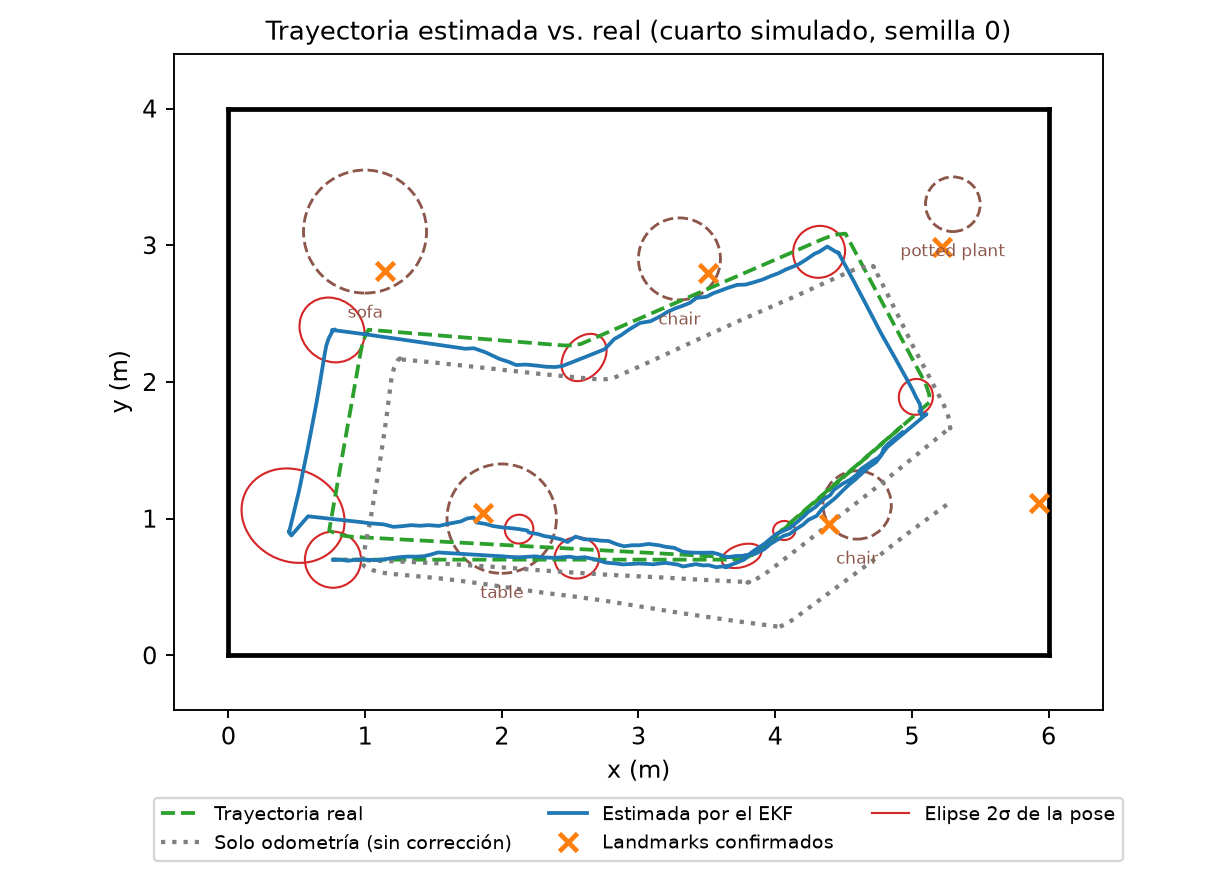
\includegraphics[width=0.85\textwidth]{Capturas_TT2/slam_trayectorias.png}
    \caption{Trayectoria real, estimada por el EKF y solo con odometría en el cuarto
    simulado. Los círculos discontinuos son los obstáculos reales.}
    \label{fig:slam_trayectorias}
\end{figure}

La Tabla~\ref{tab:slam_semillas} reporta seis corridas con semillas aleatorias
distintas.

\begin{table}[H]
\centering
\caption{Resultados del SLAM en el banco de simulación (300 ciclos por corrida)}
\label{tab:slam_semillas}
\renewcommand{\arraystretch}{1.2}
\begin{tabular}{|c|c|c|c|c|}
\hline
\textbf{Semilla} & \textbf{ATE EKF (m)} & \textbf{ATE solo odometría (m)} &
\textbf{Error de orientación} & \textbf{Landmarks} \\
\hline
0 & 0.142 & 0.318 & $2.31^\circ$ & 6 \\
1 & 0.288 & 0.250 & $4.16^\circ$ & 7 \\
2 & 0.270 & 0.273 & $3.86^\circ$ & 6 \\
3 & 0.116 & 0.191 & $2.64^\circ$ & 7 \\
4 & 0.249 & 0.164 & $1.71^\circ$ & 6 \\
5 & 0.205 & 0.188 & $2.48^\circ$ & 8 \\
\hline
\textbf{Promedio} & \textbf{0.212} & \textbf{0.231} & $\mathbf{2.86^\circ}$ & \textbf{6.7} \\
\hline
\end{tabular}
\end{table}

Estos números hay que leerlos con cuidado. En promedio el EKF baja el error de 0.23 a
0.21~m, pero no en todas las corridas, porque en dos de las seis la odometría sola fue
más precisa. En recorridos cortos y sin sesgo, como los del banco, integrar la odometría
ya da un buen resultado, y las correcciones contra \emph{landmarks} ubicados con
distancia monocular meten un error parecido al que quitan. Con una odometría real la
historia cambia, porque la longitud de paso nunca queda perfectamente calibrada y los
sensores tienen sesgo. Para ver ese caso se repitió el experimento con recorridos de
1200 ciclos (unas cuatro vueltas al cuarto) y con odometría sesgada; los resultados están
en la Tabla~\ref{tab:slam_deriva} y en la Figura~\ref{fig:slam_deriva}.

\begin{table}[H]
\centering
\caption{ATE promedio (y máximo) en seis corridas con odometría sesgada}
\label{tab:slam_deriva}
\renewcommand{\arraystretch}{1.2}
\begin{tabular}{|p{5.6cm}|c|c|}
\hline
\textbf{Escenario} & \textbf{EKF (m)} & \textbf{Solo odometría (m)} \\
\hline
300 ciclos, sin sesgo & 0.21 (0.29) & 0.23 (0.32) \\
1200 ciclos, sin sesgo & 0.28 (0.35) & 0.42 (0.61) \\
1200 ciclos, longitud de paso +10\,\% & 0.38 (0.62) & 0.58 (0.80) \\
1200 ciclos, giro sesgado $+0.1^\circ$/ciclo & 0.89 (1.68) & 1.64 (1.86) \\
1200 ciclos, ambos sesgos & 1.34 (1.89) & 1.75 (2.01) \\
\hline
\end{tabular}
\end{table}

\begin{figure}[H]
    \centering
    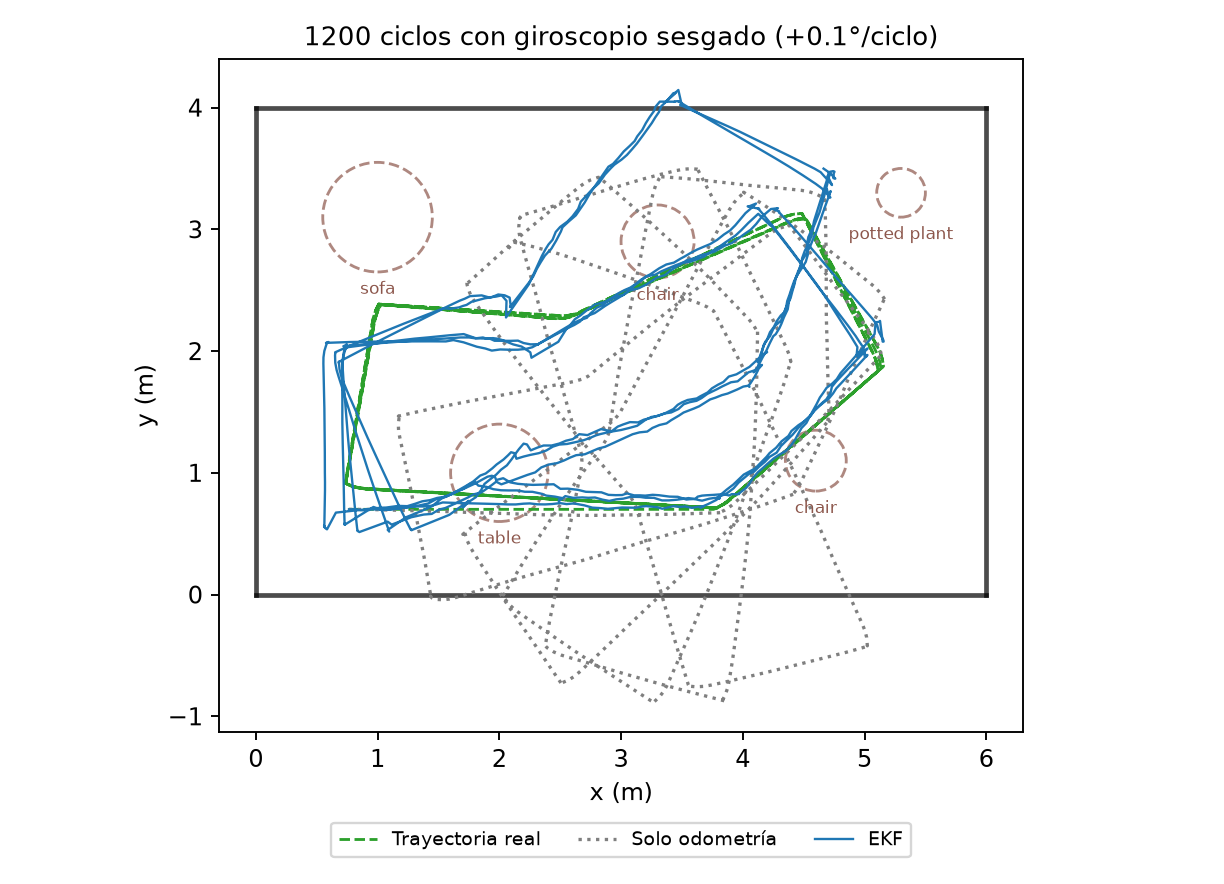
\includegraphics[width=0.78\textwidth]{Capturas_TT2/slam_deriva.png}
    \caption{Recorrido de 1200 ciclos con giroscopio sesgado (semilla 0). La odometría
    sola va girando el recorrido; el EKF lo mantiene cerca del real, aunque con
    desviaciones de hasta un metro en algunos tramos.}
    \label{fig:slam_deriva}
\end{figure}

En recorridos largos y con error de escala en el paso, el EKF reduce el error de la
odometría en alrededor de un tercio, que es justo para lo que sirve el SLAM. Con el
giroscopio sesgado lo reduce casi a la mitad en promedio, aunque el máximo llega a
1.7~m, y con los dos sesgos juntos la mejora baja a una cuarta parte. En esas corridas
se observó una divergencia de orientación, ya que en dos de las seis el error de rumbo
pasó de $100^\circ$ hacia el final. Con el rumbo tan equivocado, las detecciones dejan
de asociarse con los \emph{landmarks} que ya existen y se crean duplicados desplazados
(hasta diez sillas en un cuarto que tiene dos), y el filtro termina siendo consistente
con un mapa erróneo. Es la forma típica en que falla un EKF sin cierre de lazo.

En el prototipo este caso es poco probable, porque el giro no se integra a partir del
giroscopio sino que se toma del rumbo que entrega la BNO055 en su modo de fusión con
magnetómetro. Ese rumbo es absoluto, así que el sesgo no se va sumando como en la
simulación. Para que funcione, la brújula debe estar calibrada; por eso, al arrancar,
el sistema revisa el estado de calibración del magnetómetro y, si es bajo, le pide al
usuario que mueva los lentes en forma de ocho. El experimento sigue siendo útil por dos
razones, ya que muestra lo que pasaría con una brújula mal calibrada o alterada por
estructuras metálicas, y describe el modo de respaldo sin IMU, en el que el giro sale
del flujo óptico y sí acumula error.

\textbf{Pérdida de observaciones.} Para probar el manejo de oclusiones se repitió la
corrida de la semilla 0 quitando todas las detecciones visuales entre los ciclos 120 y
200. En la Figura~\ref{fig:slam_incertidumbre} se ve que, durante la oclusión, la traza
de la covarianza crece sin parar y la confianza cae casi a cero, es decir, el sistema se
da cuenta de que su pose ya no es fiable. En cuanto vuelve a ver objetos conocidos
(ciclo 220), la incertidumbre se reduce de golpe. El ATE de esta corrida fue de
0.08~m, así que la oclusión no hizo que el sistema se perdiera. En la corrida normal
también hay caídas de confianza en los tramos donde la cámara no tiene objetos a la
vista.

\begin{figure}[H]
    \centering
    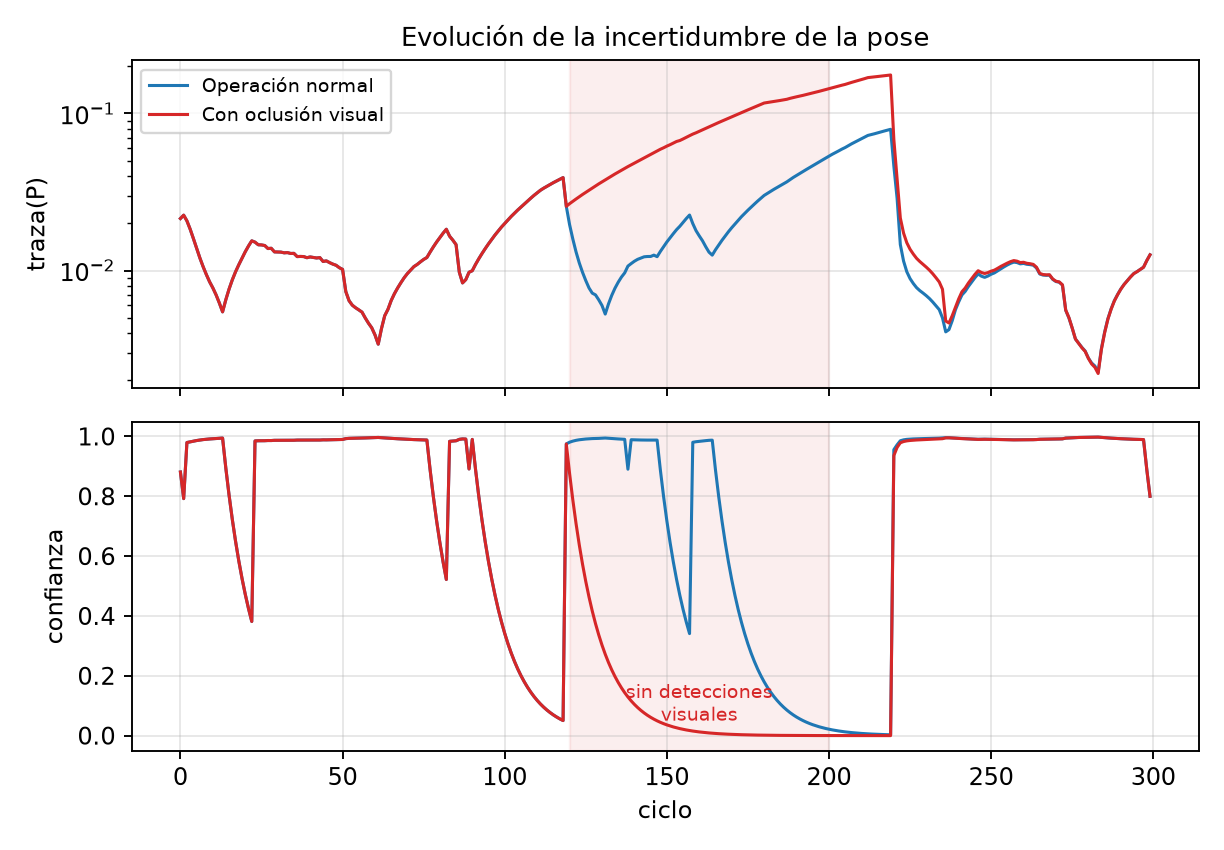
\includegraphics[width=0.85\textwidth]{Capturas_TT2/slam_incertidumbre.png}
    \caption{Evolución de la traza de la covarianza (escala logarítmica) y de la
    confianza, con y sin oclusión visual entre los ciclos 120 y 200.}
    \label{fig:slam_incertidumbre}
\end{figure}

Al quitar al azar el 60\,\% de las detecciones visuales en las seis corridas, el ATE
promedio fue de 0.23~m (máximo 0.28~m), por lo que el módulo aguanta bien las
detecciones intermitentes.

\textbf{Videos reales.} En los 19 videos grabados, el SLAM confirmó entre 1 y 39
\emph{landmarks} por recorrido. En interiores la clase más frecuente fue la puerta,
con entre 9 y 17 por recorrido de oficina. En las calles hubo muy pocos objetos
estáticos de las clases que se detectan, y en el recorrido más pobre se confirmó uno
solo, de modo que el sistema avanzó casi todo el tiempo con la pura predicción. La
Sección~\ref{sec:dev_integracion} presenta capturas del sistema trabajando con video.

\textbf{Costo computacional.} Un ciclo del EKF tarda en promedio 0.03~ms en el banco,
con unos siete \emph{landmarks}, y 0.27~ms con video real, con unos cuarenta, porque la
asociación crece linealmente con su número. En la Raspberry Pi del prototipo el ciclo
tarda \TODO{tiempo por ciclo del EKF en la Raspberry Pi}. En cualquier caso el costo es
mínimo frente a los 100~ms por ciclo que permite RNF-03.

\subsection{Limitaciones}

El rumbo absoluto de la BNO055 depende de que el magnetómetro esté calibrado y de que no
haya perturbaciones magnéticas cerca, como estructuras de acero o equipos eléctricos. La
calibración se revisa al arrancar, pero durante la sesión ningún módulo reacciona si
empeora. \TODO{avisar al usuario si la calibración del magnetómetro baja durante la
sesión}.

El filtro no hace cierre de lazo (\emph{loop closure}). Si la deriva es grande al
regresar a una zona ya visitada, el error no se reparte a lo largo de la trayectoria
anterior, y si el error de orientación rebasa lo que tolera la compuerta de asociación,
aparecen \emph{landmarks} duplicados y el filtro puede divergir. La posición de los
\emph{landmarks} monoculares depende además de la altura típica de su clase, así que un
objeto de tamaño poco común puede quedar mal ubicado, como el que aparece junto a la
pared en la Figura~\ref{fig:slam_trayectorias}. La asociación por vecino más cercano
también puede confundir dos objetos cercanos de la misma clase; una prueba de
compatibilidad conjunta \cite{neira2001jcbb} sería más confiable, a cambio de más
cómputo.

Por último, los valores de ruido de la odometría se ajustaron en simulación.
\TODO{medir el ruido real de la IMU y del conteo de pasos en el prototipo y actualizar
los parámetros del filtro}. En los mapas que se obtienen de video la escala depende de
la velocidad de caminata supuesta, porque el video no trae información de
desplazamiento.
